\chapter{ Конструкторский раздел}
\label{cha:design}
        В данном разделе будут рассмотрены описание системы, требования к функциональности ПО
        и определены способы тестирования.
    \section{Описание системы}
        Система состоит из трех этапов (рисунок \ref{schema:conveyor}),
        который последовательно соединены между собой. 
        Каждый этап выполняет возведение в квадрат
        полученного на вход элемента. 
        Для уменьшения влияния времени диспетчеризации 
        будет вызываться системный вызов sleep 
        с разным временем ожидания для каждого этапа.
        Время попадания в каждую очередь логируется.

    \begin{figure}[h!]
        \centering
            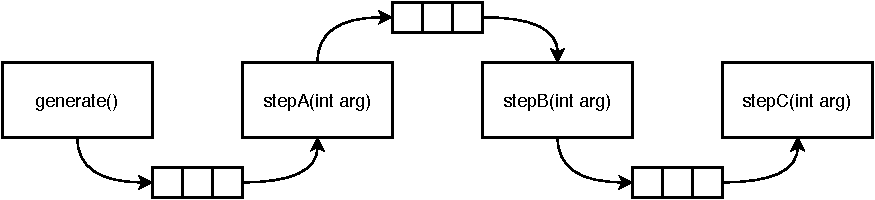
\includegraphics[scale=0.9]{schema_conveyor.pdf}
            \caption{Схема конвейерной обработки}
            \label{schema:conveyor}
    \end{figure}


    \section{Требования к функциональности ПО}
        В данной работе требуется обеспечить следующую минимальную функциональность консольного приложения:
        \begin{enumerate}
            \item предоставить возможность ввода количества генерируемых элементов в системе;
            \item обеспечить вывод времени получения и отправки элемента конвейера.
        \end{enumerate}

    \section{Тесты}
        Тестирование ПО будет проводиться методом чёрного ящика. 
        Эффект от конвейеризации становиться заметен,
        если время выполнения этапа много больше времени диспетчеризации. 
        Каждый этап будет возводить число в квадрат и вызывать системный вызов sleep 
        с разным временем ожидания для каждого этапа.

    \section{Вывод}
        В данном разделе были рассмотрены схема алгоритмов 
        обработки элементов линии конвейера и
        описаны требования к функциональности ПО.
        

\newpage